%===================================
\chapter{Représentation des données\index{Representation des données@Représentation des données}}
%====================================

	Nous voici arrivés au terme de ce cours d'algorithmique. 
	Ce chapitre apporte une synthèse des différentes notions vues 
	tout au long de vos cours d'algorithmiques de 1\iere\ année 
	et propose quelques pistes de réflexion 
	quant au choix d’une bonne représentation des données 
	qui se pose lors de la résolution de problèmes de programmation avancés.
	
	Pour la plupart de ces exercices,
	la difficulté tient en partie dans le bon choix d’une représentation des données 
	et de la démarche algorithmique la plus adéquate à mettre en \oe{}uvre 
	pour agir sur ces données en vue d’obtenir le résultat escompté. 
	Noter que l’efficacité d’un algorithme 
	est liée étroitement au choix de la représentation.

%======================================
\section{Se poser les bonnes questions}
%=======================================

	Revenons à la case départ : 
	nous avons commencé le cours d'algorithmique de DEV1
	en situant les notions de \textbf{problème} et de \textbf{résolution}. 
	Nous avons vu qu’un problème bien spécifié s’inscrit dans le schéma :
	
		\begin{center}
		\begin{Ovalbox}
			{\textbf{étant donné} [la situation de départ] 
			\textbf{on demande} [l’objectif]}
		\end{Ovalbox}
		\end{center}
	
	Une fois le problème correctement posé, 
	on peut partir à la recherche d’une \textbf{méthode de résolution}, 
	c’est-à-dire d’un algorithme en ce qui concerne les problèmes 
	à résoudre par les moyens informatiques.
	
	Tout au long de l’année, 
	nous avons vu divers modèles et techniques algorithmiques adaptés 
	à des structures particulières 
	(les nombres, les chaines, les tableaux, les variables structurées, 
	les objets, les listes\dots). 
	La plupart des exercices portaient directement sur ces structures 
	(par ex. calculer la somme des nombres d’un tableau,
	extraire une sous-liste à partir d’une liste donnée). 
	Ces exercices d’entrainement et de formation quelque peu théoriques 
	constituent en fait des démarches algorithmiques de base 
	qui trouvent toutes une place dans des problèmes plus complexes.
	
	Mais la plupart des problèmes 
	issus des situations de la vie courante 
	auxquels se confronte le programmeur 
	s’expriment généralement de manière plus floue : 
	par ex. dresser la comptabilité des dépenses mensuelles d’une firme, 
	faire un tableau récapitulatif du résultat des élections par cantons électoraux, 
	faire une version informatique d’un jeu télévisé\dots{} 
	Les exemples sont infinis !
	
	C’est dans le cadre de ce genre de problème plus complexe 
	que se pose le problème de la \textbf{représentation de données}. 
	Une fois le problème bien spécifié (par les données et l’objectif) 
	apparaissent naturellement les questions suivantes : 
	quelles données du problème sont réellement utiles à sa résolution ?
	(Il est fréquent que l’énoncé d’un problème contienne 
	des données superflues ou inutiles). 
	Y a-t-il des données plus importantes que d’autres ? 
	(données principales ou secondaires). 
	Les données doivent-elles être consultées plusieurs fois ?
	Quelles données faut-il conserver en mémoire ? Sous quelle forme ?
	Faut-il utiliser un tableau ? Une liste ? 
	Faut-il créer une nouvelle classe ? 
	Les données doivent-elles être classées suivant un critère précis ? 
	Ou la présentation brute des données suffit-elle pour
	solutionner le problème posé ?
	
	Les réponses ne sont pas directes, 
	et les différents outils qui sont à notre disposition 
	peuvent être ou ne pas être utilisés. 
	Il n’y a pas de règles précises pour répondre à ces questions, 
	c’est le flair et le savoir-faire 
	développés patiemment par le programmeur au fil de ses expériences 
	et de son apprentissage qui le guideront vers la solution la plus efficace. 
	Parfois plusieurs solutions peuvent fonctionner 
	sans pouvoir départager la meilleure d’entre elles.
	
	Ce type de questionnement est peut-être l’aspect le plus délicat 
	et le plus difficile de l’activité de programmation, 
	car d’une réponse appropriée dépendra toute l’efficacité du code développé. 
	Un mauvais choix de représentation des données 
	peut mener à un code lourd et maladroit. 
	En vous accompagnant dans la résolution des exercices qui suivent,
	nous vous donnerons quelques indices et pistes de réflexion, 
	qui seront consolidées par l’expérience acquise 
	lors des laboratoires de langages informatiques 
	ainsi que par les techniques de modélisation vues au cours d’analyse.

%==================================
\section{Les structures de données\index{Structures de donnees@Structures de données}}
%==================================

	Rappelons brièvement les différentes structures étudiées dans ce cours
	\index{Structures a connaitre@Structures à connaitre} :
	
	\begin{itemize}
		\item 
			les \textbf{données «~simples~»} 
			(variables isolées : entiers, réels, chaines, caractères, booléens) ;
		\item 
			les \textbf{variables structurées}, 
			qui regroupent en une seule entité
			une collection de variables simples ;
		\item 
			le \textbf{tableau}, 
			qui contient un nombre déterminé de variables de même type, 
			accessibles via un indice 
			ou plusieurs pour les tableaux multidimensionnels ;
		\item 
			les \textbf{objets}, 
			qui combinent en un tout une série d’attributs 
			et des méthodes agissant sur ces attributs ;
		\item 
			la \textbf{Liste}, 
			qui peut contenir un nombre indéfini d’éléments de même type.
	\end{itemize}
	
	D’autres structures particulières s’ajouteront 
	dans le cours d'algorithmique de DEV4~: 
	les listes chainées, les piles, les files, les arbres et les graphes.
	
	Chacune de ces structures possède ses spécificités propres quant à la
	façon d’accéder aux valeurs, de les parcourir, de les modifier,
	d’ajouter ou de supprimer des éléments à la collection. 

\clearpage
%==================
\section{Exercices}
%==================

%---------------------------------------------------
\begin{Exercice}{La course à la case 64 à 4 joueurs}
%---------------------------------------------------
	Commençons par un petit jeu très simple de course avec un dé, dont voici les règles.
	
	\begin{quote}
	\og Ce jeu se joue à $n$ joueurs qui doivent parcourir un chemin de 64 cases.
	Ils commencent tous sur la case 1 et jouent à tour de rôle
	(en commençant par le premier joueur).
	À son tour, le joueur lance un dé à 6 faces 
	et avance du nombre de cases indiqué par le dé.
	Le premier joueur à atteindre ou dépasser la case 64 a gagné.
	Seule contrainte, un joueur ne peut pas terminer son tour
	sur une case occupée. 
	Si c'est le cas, il avance jusqu'à la case libre suivante.\fg
	\end{quote}
	
	Voici 3 propositions de représentation de données. 
	On vous demande pour chaque proposition de vérifier, 
	sans écrire l'algorithme, si elle permet la programmation du jeu. 
	On vous conseille vivement de \og{}dessiner\fg{}%
	\footnote{
		Par là, on veut dire : imaginer une situation de jeu
		(positions des joueurs sur le chemin par exemple)
		et voir quelles valeurs doivent avoir les variables
		introduites dans la représentation pour correspondre
		à cette situation de jeu. 
	} les propositions
	pour mieux les comprendre.
	
	\begin{enumerate}
	\item 
		Un tableau de 64 entiers.
		La case $k$ contient $i$ si le joueur $i$ s'y trouve 
		ou $0$ si la case est libre.
		Mais aussi un entier \lda{joueurCourant} donnant
		le numéro du joueur courant.
	\item
		Un tableau de 4 entiers. 
		La case i contient la position du joueur i.
		Mais aussi un entier \lda{joueurCourant} donnant
		le numéro du joueur courant.
	\item
		On combine les deux premières propositions
		(on a donc deux tableaux).
	\end{enumerate}

	Après ces vérifications vous choisirez une des représentations 
	pour écrire la solution du jeu sous forme d'une classe \lda{Course64}.
	Pensez à découper votre solution.
	
\end{Exercice}

%---------------------------------------------------
\begin{Exercice}{La course à la case 64 à n joueurs}
%---------------------------------------------------

	Modifiez l'exercice précédent 
	afin que le jeu puisse se jouer à $n$ joueurs,
	où $n$ est un entier supérieur ou égal à 2, choisi au début du jeu.

\end{Exercice}
	
%-------------------------------------------------
\begin{Exercice}{La course à la case 64 à n joueurs - variantes}
%-------------------------------------------------

	Reprenons la course à la case 64 de l'exercice précédent.
	Voici quelques propositions de modification des règles.
	Pour chaque proposition, indiquez si la représentation
	choisie dans l'exercice précédent est toujours valable et pertinente.
	\begin{enumerate}
	\item 
		Si un joueur arrive sur une case occupée, 
		le joueur qui s'y trouvait retourne à la première case.
	\item
		Si un joueur termine sa course sur une case qui est un multiple de 5,
		il rejoue directement.
	\item
		Un joueur rejoue directement s'il termine sa course
		sur les cases 1, 2, 7, 11, 17, 31, 42 ou 53.
	\end{enumerate}
	
\end{Exercice}

%------------------------------------
\begin{Exercice}{Un jeu de poursuite}
%------------------------------------

	Deux joueurs A et B se poursuivent sur un circuit de 50 cases. 
	Au départ, A se trouve sur la case 1 et B est placé sur la case 26.
	C’est A qui commence. 
	Chaque joueur joue à son tour en lançant un dé dont la valeur 
	donne le nombre de cases duquel il doit avancer sur le jeu. 
	Lorsqu’un joueur arrive sur la case 50 et qu’il doit encore avancer, 
	il continue son parcours à partir de la case 1. 
	Le jeu se termine lorsqu’un joueur rattrape ou dépasse l’autre.

	Écrire un algorithme de simulation de ce jeu
	qui se terminera par l’affichage du vainqueur ainsi que le nombre de
	tours complets parcourus par ce vainqueur. 

	La solution se trouvera dans une classe \lda{JeuPoursuite}
	qui contiendra les méthodes suivantes :
	\begin{itemize}
		\item 
			Le constructeur.
		\item 
			La méthode \lda{initialiser()} initialise le jeu
			(placement des joueurs\dots).
		\item 
			La méthode \lda{jouer()} lance le jeu jusqu’à son terme et
			donne le vainqueur et le nombre de tours effectués par chacun.
		\item 
			Vous êtes également fortement invités à définir d’autres méthodes en
			privé pour modulariser au mieux votre code. 
			Par exemple, on pourrait définir :
			\begin{itemize}
				\item 
					la méthode \og{}\lda{~jouerCoup~}\fg{} qui joue pour un joueur et
					indique s'il a rattrapé l’autre joueur
				\item 
					la méthode \og{}\lda{~joueurSuivant~}\fg{} qui permet de passer au
					joueur suivant.
			\end{itemize}
			Avec ces méthodes, la méthode publique \og{}\lda{~jouer~}\fg{} 
			devient triviale.
	\end{itemize}

	À nouveau, on vous fait plusieurs propositions pour la représentation
	de l'état du jeu.
	On vous demande pour chacune d'elles de vérifier, 
	sans écrire les méthodes de la classe, 
	si elles permettent la programmation du jeu. 
	Après ces vérifications vous choisirez 
	une des représentations pour écrire la classe complète.
	
	\begin{itemize}
	\item 
		Dans cette proposition, nous avons deux attributs.
		\begin{itemize}
		\item 
			\lda{circuit}~: un tableau de 1 à 50 chaines de caractères. 
			Les chaines de caractères représenteront la position des joueurs 
			(au départ, "A" en 1 et "B" en 26, " " dans les autres positions).
		\item
			\lda{joueurCourant}~: un entier donnant la position du joueur courant.
		\end{itemize}
	\item
		Cette proposition introduit une structure \lda{Joueur} et le nombre de tours.
		\begin{itemize}
		\item
			\lda{circuit}: un tableau de 1 à 50 éléments \lda{Joueur}.  
			La structure \lda{Joueur} est composée d'un nom (chaine) 
			et d'un nombre de tours (entier).			
			Joueur reprendra le nom du joueur à cette position 
			("A", "B" ou " " si la case est vide); 
			nbTour donne le nombre de tours qu'a fait le joueur qui est à cette position 
			(0 si la case est vide).
			Un joueur a fait un tour complet quand il a est de nouveau sur sa position de départ
			ou la dépasse.
		\item
			\lda{joueurCourant}: un entier donnant la position du joueur courant.
		\end{itemize}
	\item
		Dans cette proposition, le tableau change de signification
		\begin{itemize}
		\item
			\lda{circuit}: un tableau de 2 éléments \lda{Joueur}.  
			La structure \lda{Joueur} est composée 
			de position: entier et nbTour: entier 
			où position donne la position du joueur sur le circuit 
			(entier entre 1 et 50) 
			et nbTour donne le nombre de tours qu'a fait le joueur.
		\item
			\lda{joueurCourant}: un entier donnant la position du joueur courant.
		\end{itemize}
	\item
		Dans cette proposition, la structure est remplacée par une classe
		contenant les mêmes données mais introduisant des méthodes.
		\begin{itemize}
		\item
			\lda{circuit}: un tableau de 2 éléments \lda{Joueur}.  
			La structure \lda{Joueur} est composée 
			de position: entier et nbTour: entier 
			où position donne la position du joueur sur le circuit 
			(entier entre 1 et 50) 
			et nbTour donne le nombre de tours qu'a fait le joueur.
		\item
			\lda{joueurCourant}: un entier donnant la position du joueur courant.
		\end{itemize}
	\item
		Cette proposition est fort proche de la précédente mais, cette fois,
		un joueur reprendra plutôt le numéro de la case de départ
		et le nombre de cases parcourues.
	\end{itemize}
	
\end{Exercice}

%-----------------------------------------------
\begin{Exercice}{Un jeu de poursuite - variante}
%-----------------------------------------------

	Dans cette variante,
	chaque case contient une valeur vrai ou faux
	indiquant si le joueur pourra rejouer.
	Si la case sur laquelle tombe le joueur contient la valeur
	\lda{vrai} il avance encore une fois du même nombre de cases 
	(et de même s’il tombe encore sur \lda{vrai}).
	
			Le constructeur reçoit la configuration du circuit 
			(pour savoir si les cases contiennent \lda{vrai} ou \lda{faux})

	Qu'est-ce que cela change au niveau des données ?
	Modifiez la classe \lda{JeuPoursuite en conséquence}.
	
	Pour le code, 
	nous vous conseillons de ne pas modifier la méthode \lda{jouerCoup} 
	mais de la rendre privée et d'introduire une méthode qui y fait appel
	plusieurs fois si nécessaire.
\end{Exercice}

%---------------------------------------
\begin{Exercice}{Le Jeu du Millionnaire}
%---------------------------------------

	Un questionnaire de quinze questions à choix
	multiples de difficulté croissante est soumis à un candidat. Quatre
	possibilités de réponses (dont une seule est correcte) sont proposées à
	chaque fois. Au plus le candidat avance dans les bonnes réponses, au
	plus son gain est grand. S’il répond correctement aux quinze questions,
	il empoche la somme rondelette de 500.000~\texteuro.
	
	Par contre, si le candidat donne une mauvaise
	réponse, il risque de perdre une partie du gain déjà acquis. Cependant,
	certains montants intermédiaires constituent des paliers, c’est-à-dire
	une somme acquise que le candidat est sûr d’empocher, quoiqu’il arrive
	dans la suite du jeu.

	À chaque question, le candidat a donc trois
	possibilités~:
	\begin{itemize}
		\item 
			il donne la réponse correcte : dans ce cas il
			augmente son gain, et peut passer à la question suivante
		\item 
			il ne connait pas la réponse, et choisit de
			s’abstenir : dans ce cas, le jeu s’arrête et le candidat empoche le
			gain acquis à la question précédente
		\item 
			il donne une réponse incorrecte : le jeu
			s’arrête également, mais le candidat ne recevra que le montant du
			dernier palier qu’il a atteint et réussi lors de son parcours. En
			particulier, si le candidat se trompe avant d’avoir atteint le premier
			palier, il ne gagne pas un seul euro !
	\end{itemize}
	
	\begin{minipage}[t][][b]{2.5cm}
	\begin{center}
	\begin{footnotesize}
	\begin{tabular}{|l|l|l|}\hline
	  1 &      25~\texteuro & faux \\\hline
	  2 &      50~\texteuro & faux \\\hline
	  3 &     125~\texteuro & faux \\\hline
	  4 &     250~\texteuro & faux \\\hline
	  5 &     500~\texteuro & vrai \\\hline
	  6 &    1000~\texteuro & faux \\\hline
	  7 &    2000~\texteuro & faux \\\hline
	  8 &    3750~\texteuro & faux \\\hline
	  9 &    7500~\texteuro & faux \\\hline
	 10 &   12500~\texteuro & vrai \\\hline
	 11 &   25000~\texteuro & faux \\\hline
	 12 &   50000~\texteuro & faux \\\hline
	 13 &  100000~\texteuro & vrai \\\hline
	 14 &  250000~\texteuro & faux \\\hline
	 15 &  500000~\texteuro & vrai \\\hline
	\end{tabular}
	\end{footnotesize}
	\end{center}
	\end{minipage}%
	\hfill
	\begin{minipage}[t][][b]{10cm}
	Exemple : Le tableau ci-contre contient les gains associés à chaque 
	question et une indication booléenne mise à
	\lda{vrai} lorsque la question
	constitue un palier. Un concurrent qui se
	trompe à la question 3 ne gagnera rien ; un concurrent qui se trompe à
	la question 6 gagnera 500~\texteuro{} (palier de la question 5) et de même s’il
	se trompe à la question 10 ; un concurrent qui se trompe à la question
	13 gagnera 12500~\texteuro{} (palier de la question 10) ; 
	s'il décide de ne pas répondre à la question 13,
	il garde le montant acquis à la question 12, soit 50000~\texteuro.
	\end{minipage}
	
	Il y aurait de nombreuses façons de coder ce problème; en voici une :

	{\bfseries La structure Question}

	Une question est composée du libellé de la question, des 4 libellés pour
	les réponses et d’une indication de la bonne réponse (un entier de 1 à
	4). Par simplicité on en fait une structure mais on pourrait en faire
	une classe si on voulait par exemple vérifier que la «~bonne réponse~»
	possède une valeur correcte.

	{\bfseries La structure Gain}

	Représente un niveau de gain. Elle contient les champs :
	montant (entier) et palier (un booléen à
	\lda{vrai} si cette somme est
	assurée, \lda{faux} sinon)

	{\bfseries La classe Millionnaire}

	Cette classe code le moteur du jeu. On y retrouve

	\begin{itemize}
		\item 
			questionnaire : un tableau de Question
		\item 
			gains : un tableau de Gain
		\item 
			autres attributs à déterminer (cf. méthodes)
	\end{itemize}
	
	ainsi que les méthodes pour

	\begin{itemize}
		\item 
			initialiser le jeu à partir d’un questionnaire
			et du tableau de gains
		\item 
			connaitre la question en cours
		\item 
			donner la réponse du candidat à la question en
			cours
		\item 
			savoir si le jeu est fini ou pas
		\item 
			arrêter le jeu en repartant avec les gains
		\item 
			les accesseurs nécessaires pour connaitre
			l’état du jeu.
	\end{itemize}
	
	{\bfseries
	Le jeu proprement dit}

	L'algorithme \lda{jeuMillionaireConsole()} reçoit le
	questionnaire et les gains et simule le jeu :

	\begin{itemize}
	\item 
		Il propose les questions au candidat
	\item 
		Il lit ses réponses (chiffre 1 à 4 ou 0 pour
		arrêter) et fait évoluer le jeu en fonction.
	\item 
		lorsque le jeu est terminé, il indique au
		candidat le montant de ses gains.
	\item 
		Attention ! Cet algorithme devrait être le plus
		petit possible. Imaginez que vous devez également coder une version
		graphique. Tout code commun doit se trouver dans la classe
	\lda{Millionnaire~}!
	\end{itemize}
\end{Exercice}

%---------------------------------
\begin{Exercice}{Chambre avec vue}
%---------------------------------

	Un grand hôtel a décidé d’informatiser sa
	gestion administrative. Il a confié ce travail à la société ESI\_INFO
	dans laquelle vous êtes un informaticien chevronné. On vous a confié la
	tâche particulière de la gestion des réservations pour ses 100
	chambres.
	Pour ce faire, on vous demande d’écrire une
	classe \lda{Hôtel} qui offre
	notamment une méthode qui permet d’enregistrer une réservation.

	Pour représenter l’occupation des chambres un
	jour donné, nous allons utiliser un tableau de 100 entiers. Un 0
	indique que la chambre est libre, une autre valeur (positive) indique
	le numéro du client qui occupe cette chambre ce jour-là.

	Nous utiliserons une Liste de tels tableaux
	pour représenter l’occupation des chambres sur une longue période ; les
	éléments se suivant correspondant à des jours successifs. 

	Nous vous imposons les attributs de la classe,
	à savoir :

	\begin{itemize}
		\item 
			\lda{occupations~}: une Liste de
			tableaux de 100 entiers comme expliqué ci-dessus.
		\item 
			\lda{premierJour~}: donne le
			jour concerné par le premier élément de la liste. Ainsi
			s'il vaut 10/9/2015 cela signifie que le premier
			élément de la liste «~occupations~» renseigne sur l’occupation des
			chambres ce 10/9/2015 ; que le deuxième élément de la liste concerne le
			11/9/2015 et ainsi de suite...
	\end{itemize}
	
	Écrire la méthode suivante

	\begin{LDA}
		\Entete{effectuerRéservation}{demande\In : DemandeRéservation,
		chambre\Out : entier}{booléen}
	\end{LDA}
	
	où la structure de demande de réservation est
	définie ainsi
	
	\begin{LDA}
		\Struct{DemandeRéservation}
			\Decl{numéroClient}{entier}
			\Decl{débutRéservation}{Date}
			\Decl{nbNuitées}{entier}
		\EndStruct
	\end{LDA}

	\begin{itemize}
		\item 
			Le booléen retourné indique si la réservation a pu se faire ou pas
		\item 
			Si elle a pu se faire, le paramètre de sortie
			\lda{chambre} indique la chambre qui a été choisie
		\item 
			Si plusieurs chambres sont libres, on choisit celle avec le plus petit
			numéro
		\item 
			La demande de réservation peut couvrir une période qui n’est pas encore
			reprise dans la liste ; il faudra alors l’agrandir
	\end{itemize}
\end{Exercice}

%---------------------------
\begin{Exercice}{L'ensemble}
%---------------------------

	La notion d’ensemble fini est une notion qui vous est déjà 
	familière pour l’avoir rencontrée dans plusieurs cours. Nous rappelons
	certaines de ses propriétés et opérations. 
			
	Étant donnés deux ensembles
	finis \textbf{S} et \textbf{T} ainsi qu’un élément \textbf{x} :

	\begin{itemize}
	\item 
		\textbf{x} {${\in}$} \textbf{S} signifie que l’élément \textbf{x}
		est un élément de l’ensemble \textbf{S}.
	\item 
		L’ensemble vide, noté \textbf{${\emptyset}$} 
		est l’ensemble qui n’a pas d’élément 
		(\textbf{x} {${\in}$} \textbf{${\emptyset}$} 
		est faux quel que soit \textbf{x} ).
	\item 
		L’ordre des éléments dans un ensemble n’a
		aucune signification, l’ensemble \{1,2\} est
		identique à \{2,1\}.
	\item 
		Un élément \textbf{x} ne peut
		pas être plus d’une fois élément d’un même ensemble 
		(pas de répétition).
	\item 
		L’union \textbf{S ${\cup}$ T} 
		est l’ensemble contenant les éléments qui sont dans 
		\textbf{S} ou (non exclusif) dans \textbf{T}.
	\item 
		L’intersection \textbf{S ${\cap}$ T} 
		est l’ensemble des éléments qui sont à la fois 
		dans \textbf{S} et dans \textbf{T}.
	\item 
		La différence \textbf{S {\textbackslash} T} 
		est l’ensemble des éléments qui sont 
		dans \textbf{S} mais pas dans \textbf{T}.
	\end{itemize}
	
	Créer la classe \lda{Ensemble}
	décrite ci-dessous.
	
	\begin{LDA}
		\Class{Ensemble de E}{} 
		\RComment E est le type des éléments de l'ensemble
		
			\Public
			\ConstrSign{Ensemble de E}{} 
			\RComment construit un ensemble vide
			\MethodSign{ajouter}{élt : E}{}
			\RComment ajoute l'élément à l'ensemble
			\MethodSign{enlever}{élt : E}{})
			\RComment enlève un élément de l'ensemble
			\MethodSign{contient}{élt : E}{booléen}
			\RComment dit si l'élément est présent
			\MethodSign{estVide}{}{booléen}
			\RComment dit si l'ensemble est vide
			\MethodSign{taille}{}{entier}
			\RComment donne la taille de l'ensemble
			\MethodSign{union}{autreEnsemble : Ensemble de E}{Ensemble de E}
			\MethodSign{intersection}{autreEnsemble : Ensemble de E}{Ensemble de E}
			\MethodSign{moins}{autreEnsemble : Ensemble de E}{Ensemble de E}
			\MethodSign{éléments}{}{Liste de E}
			\RComment conversion en liste
		\EndClass
	\end{LDA}
		
	\medskip
	Quelques remarques :
	\begin{itemize}
		\item 
			La méthode d'ajout (resp. de suppression) n'a
			pas d'effet si l'élément est déjà
			(resp. n'est pas) dans l'ensemble.
		\item 
			Les méthodes \lda{union()}, 
			\lda{intersection()} et 
			\lda{moins()} retournent un troisième ensemble, 
			résultat des 2 premiers sans toucher
			à ces 2 ensembles. On aurait pu envisager des méthodes modifiant
			l'ensemble sur lequel on les appelle.
		\item 
			La méthode \lda{éléments()}
			est nécessaire si on veut parcourir les éléments de
			l'ensemble (par exemple pour les afficher).
	\end{itemize}
	
\end{Exercice}

%---------------------------
\begin{Exercice}{Les congés}
%---------------------------

	Les périodes de congés des différents employés d’une firme sont reprises
	dans un tableau booléen \textbf{Congés} bidimensionnel à \textit{n}
	lignes et 366 colonnes. Chaque ligne du tableau correspond à un employé
	et chaque colonne à un jour de l’année. Une case de ce tableau est mise
	à \textbf{vrai} si l’employé correspondant est en congé le jour
	correspondant. La firme en question est opérationnelle 7 jours sur 7,
	on n’y fait donc pas de distinction entre jours ouvrables, week-end et
	jours fériés.

	Ce tableau permet de visualiser l’ensemble des congés des travailleurs,
	et d’accorder ou non une demande de congé, suivant les règles suivantes :
	\begin{enumerate}
		\item 
			une période de congé ne peut excéder 15 jours ;
		\item 
			un employé a droit à maximum 40 jours de congé par an ;
		\item 
			à tout moment, 50\% des employés doivent être présents dans la firme.
	\end{enumerate}
	
	Écrire un algorithme qui détermine si cette demande peut être accordée
	ou non à un employé dont on connait le nom, ainsi que les dates de
	début et de fin d’une demande de congé (objets de la classe Date). Dans
	l’affirmative, le tableau \textbf{Congés} sera mis à jour.

	Pour établir la correspondance entre ce tableau et les noms des
	employés, vous avez à votre disposition un tableau \textbf{Personnel}
	de chaines. L’emplacement du nom d’un employé dans ce tableau
	correspond à l’indice ligne du tableau \textbf{Congés}.

	Il est permis d’utiliser pour résoudre cet exercice la méthode suivante
	de la classe Date, sans devoir détailler son code :
	
	\begin{LDA}
		\Entete{numéroJour}{}{entier}
		\RComment la position du jour dans l’année (entre 1 et 366)
	\end{LDA}
\end{Exercice}

%-----------------------
\begin{Exercice}{Casino}
%-----------------------

	Pour cet exercice,
	on vous demande un petit programme qui simule un jeu de roulette
	très simplifié dans un casino.
	
	Dans ce jeu simplifié, vous pourrez miser une certaine somme 
	et gagner ou perdre de l'argent (telle est la fortune, au casino !). 
	Quand vous n'avez plus d'argent, vous avez perdu.

	\textbf{Notre règle du jeu}

	Bon, la roulette, c'est très sympathique comme jeu, 
	mais un peu trop compliqué pour un exercice de première année.
	Alors, on va simplifier les règles et je vous présente tout de suite 
	ce que l'on obtient :
	\begin{itemize}
	\item
		Le joueur mise sur un numéro compris entre 0 et 49 (50 numéros en tout). 
		En choisissant son numéro, il y dépose la somme qu'il souhaite miser.
	\item
		La roulette est constituée de 50 cases allant naturellement de 0 à 49. 
		Les numéros pairs sont de couleur noire, 
		les numéros impairs sont de couleur rouge. 
		Le croupier lance la roulette, 
		lâche la bille et quand la roulette s'arrête, 
		relève le numéro de la case dans laquelle la bille s'est arrêtée. 
		Dans notre programme, nous ne reprendrons pas tous ces détails 
		« matériels » mais ces explications sont aussi à l'intention 
		de ceux qui ont eu la chance d'éviter les salles de casino jusqu'ici. 
		Le numéro sur lequel s'est arrêtée la bille est, naturellement, 
		le numéro gagnant.
	\item
		Si le numéro gagnant est celui sur lequel le joueur a misé 
		(probabilité de 1/50, plutôt faible), 
		le croupier lui remet 3 fois la somme misée.
	\item
		Sinon, le croupier regarde si le numéro misé par le joueur 
		est de la même couleur que le numéro gagnant 
		(s'ils sont tous les deux pairs ou tous les deux impairs). 
		Si c'est le cas, le croupier lui remet 50\% de la somme misée. 
		Si ce n'est pas le cas, le joueur perd sa mise.
	\end{itemize}
	
	Dans les deux scénarios gagnants vus ci-dessus 
	(le numéro misé et le numéro gagnant sont identiques ou ont la même couleur), 
	le croupier remet au joueur la somme initialement misée avant d'y ajouter ses gains. 
	Cela veut dire que, dans ces deux scénarios, le joueur récupère de l'argent. 
	Il n'y a que dans le troisième cas qu'il perd la somme misée.
	
	Comme vous pouvez le constater,
	on ne vous fait pas de proposition pour la représentation des données.
	À vous de joueur !
\end{Exercice}

%-----------------------------
\begin{Exercice}{Mots croisés}
%-----------------------------

	Voici une grille de mots croisés.
	(on ne s'intéresse pas ici aux définitions).
	Écrire une classe \lda{Grille} offrant les méthodes
	suivantes :
	\begin{itemize}
		\item 
			placer une lettre à un endroit de la grille 
			(une case non noire bien sûr) ;
		\item 
			donner le nombre de cases noires sur la grille ;
		\item 
			donner le nombre total de mots (plus d'une lettre) de la grille 
			(donc y compris ceux que le
			joueur n’a pas encore complétés) ; 
		\item 
			donner le nombre de mots déjà complétés par le joueur.
	\end{itemize}

	\medskip
	\begin{minipage}[t][][t]{6cm}
	Exemple : dans la grille ci-contre, le nombre de cases noires est 14, le
	nombre total de mots de la grille est 37 (19 horizontaux et 18
	verticaux) et le nombre de mots déjà complétés par le joueur est 6.
	\end{minipage}
	~
	\begin{minipage}[t][][b]{8cm}	
	\begin{footnotesize}
	\begin{center}
	\begin{tabular}{|*{10}{>{\centering\arraybackslash}m{0.30cm}|}}
	\hline
	~ & ~ & A & ~ & ~ & ~ & \cellcolor{gray!50} & ~ & ~ & ~ \\\hline
	~ & ~ & L & ~ & \cellcolor{gray!50} & ~ & ~ & ~ & ~ & ~ \\\hline
	L & O & G & I & Q & U & E & \cellcolor{gray!50} & ~ & ~ \\\hline
	~ & ~ & O & \cellcolor{gray!50} & ~ & ~ & ~ & \cellcolor{gray!50} & ~ & ~ \\\hline
	\cellcolor{gray!50} & ~ & R & ~ & \cellcolor{gray!50} & ~ & \cellcolor{gray!50} & ~ & ~ & ~ \\\hline
	E & S & I & \cellcolor{gray!50} & O & ~ & H & ~ & \cellcolor{gray!50} & ~ \\\hline
	~ & \cellcolor{gray!50} & T & A & B & L & E & A & U & \cellcolor{gray!50} \\\hline
	~ & ~ & H & \cellcolor{gray!50} & J & ~ & B & ~ & ~ & ~ \\\hline
	~ & ~ & M & ~ & E & ~ & \cellcolor{gray!50} & ~ & ~ & ~ \\\hline
	~ & ~ & E & ~ & T & ~ & ~ & ~ & ~ & ~ \\\hline
	\end{tabular}
	\end{center}
	\end{footnotesize}
	\end{minipage}
	
	%Un tableau \lda{grille} à 10 lignes et 10 colonnes contient les données
	%relatives à un jeu de mots croisés simulé sur ordinateur. Chaque
	%élément de ce tableau est une structure \lda{Case},
	%contenant les deux champs :

	%\begin{itemize}
		%\item 
			%\lda{noir} : variable booléenne affectée à
			%\lda{vrai} si la case correspondant de la grille est une
			%case noire;
		%\item 
			%\lda{lettre} : contient soit le caractère inscrit par le
			%joueur dans une case, soit le caractère «~espace~» (‘ ‘) si la case est
			%encore blanche; lorsque \lda{noir} est vrai, le contenu
			%de \lda{lettre} est indéterminé et ne peut donc être
			%utilisé. 
	%\end{itemize}
		
\end{Exercice}

%----------------------------
\begin{Exercice}{Puissance 4}
%----------------------------

	Le jeu de puissance 4 se déroule dans un tableau vertical comportant 6
	rangées et 7 colonnes dans lequel deux joueurs introduisent tour à tour
	des jetons (rouges pour l’un, jaunes pour l’autre). Avec l’aide de la
	gravité, les jetons tombent toujours le plus bas possible dans les
	colonnes où on les place. Le jeu s’achève lorsqu’un des joueurs a
	réussi à aligner 4 de ses jetons horizontalement, verticalement ou en
	oblique, ou lorsque les deux joueurs ont disposé chacun leur 21 jetons
	sans réaliser d’alignement (match nul).

	\begin{minipage}[t][][b]{4cm}
	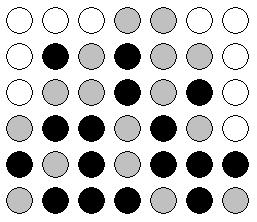
\includegraphics[width=0.8\textwidth]{image/puissance4}
	\end{minipage}
	\begin{minipage}[t][][b]{10cm}
	N.B. : sur ce dessin noir et
	blanc, les jetons rouges apparaissent en noir, les jetons jaunes en
	gris et les cases blanches désignent l'absence de
	jetons. Cet exemple montre une situation du jeu où le joueur «~jaune~»
	est gagnant. En introduisant un jeton dans la
	4\textsuperscript{e} colonne,
	il a réalisé un alignement de 4 jetons en oblique.
	\end{minipage}
	
	On demande d’implémenter une classe Puissance4 qui permette de contrôler
	l’état des différentes phases du jeu. Déterminez les attributs de cette
	classe et décrivez-les brièvement de manière à justifier votre choix.
	Dotez ensuite la classe des méthodes permettant de :

	\begin{itemize}
		\item 
			savoir si la grille est pleine
		\item 
			mettre la grille à jour lorsque le joueur n (1 ou 2) joue dans la
			colonne j (entre 1 et 7). Cette méthode renverra la valeur booléenne
			faux si la colonne en question est déjà pleine
		\item 
			vérifier si le joueur qui vient de jouer dans la colonne j a gagné la
			partie
	\end{itemize}
	
	N.B. : pour la structure qui contiendra le contenu du tableau de jetons,
	on adoptera la convention suivante : 0 pour l’absence de jeton, 1
	représentera un jeton du 1\textsuperscript{er} joueur, et 2 un jeton du
	2\textsuperscript{e} joueur (on peut donc faire abstraction de la
	couleur du jeton dans ce problème).
	
\end{Exercice}

\begin{Exercice}{Mastermind}
	Revenons sur le jeu Mastermind déjà vu en DEV1.
	Dans ce jeu, un joueur A doit trouver une combinaison de
	\lda{k} pions de couleur, choisie et tenue secrète
	par un autre joueur B. Cette combinaison peut contenir éventuellement
	des pions de même couleur. À chaque proposition du joueur A, le joueur
	B indique le nombre de pions de la proposition qui sont corrects et
	bien placés et le nombre de pions corrects mais mal placés. 

	\textbf{Exemple}

	Utilisons des lettres pour représenter les couleurs.
	
	\begin{minipage}{5cm}
		\begin{center}
		Combinaison secrète
		
		\begin{tabular}{|*{5}{>{\centering\arraybackslash}m{0.35cm}|}}
			\hline
			R & R & V & B & J \\
			\hline
		\end{tabular}
		\end{center}	
	\end{minipage}
	\
	\begin{minipage}{5cm}
		\begin{center}
		Proposition du joueur
	
		\begin{tabular}{|*{5}{>{\centering\arraybackslash}m{0.35cm}|}}
			\hline
			R & V & B & B & V \\
			\hline
		\end{tabular}
		\end{center}
	\end{minipage}
	
	Il sera indiqué au joueur qu'il a :
	\begin{itemize}
	\item 2 pions bien placés : le R en 1\iere{} position et le
	second B en 4\ieme{} position ;
	\item 1 pion mal placé : un des deux V (ils ne peuvent compter tous les deux).
	\end{itemize}
	
	\medskip
	Supposons une énumération \lda{Couleur} avec toutes les couleurs possibles de
	pion.

	\begin{enumerate}[label=\alph*)]
		\item
			Écrire une classe «\lda{~Combinaison~}» pour
			représenter une combinaison de \lda{k} pions. Elle
			possède une méthode pour générer une combinaison aléatoire (que vous ne
			devez pas écrire) et une méthode pour comparer une combinaison à la
			combinaison secrète (que vous devez écrire)
		\item
			Écrire ensuite une classe «\lda{~MasterMind~}» qui
			représente le jeu et permet d’y jouer. La taille de la combinaison et
			le nombre d’essais permis seront des paramètres du constructeur.
	\end{enumerate}
\end{Exercice}




